\chapter{Драйвер GPIO}
\textbf{Цель:} Управление выводами через встроенные в ядро драйверы и написание своего драйвера, для работы с выводами.

\vspace{5mm}
\textbf{Описание:}В предыдущей работе мы узнали, как можно управлять выводами через виртуальную файловую систему sysfs. Однако, при работе с внешними модулями, помимо интерфейса для передачи данных, могут понадобиться выводы, для управления состоянием модуля (сигнал сброса), или для проверки события (вывод ALARM на некоторых промышленных устройствах). Так же нам могут понадобиться выводы для индикации, или ввода информации. В этой работе Вы узнаете, как можно работать с выводами общего назначения через стандартные драйверы ядра, и как ими пользоваться в своих драйверах. 

\vspace{5mm}
\textbf{Полезные ссылки:}
\begin{itemize}
	\item \href{https://www.kernel.org/doc/Documentation/devicetree/bindings/input/gpio-keys.txt}{Kernel Doc: GPIO Keys}.
	\item \href{https://www.kernel.org/doc/Documentation/devicetree/bindings/leds/common.yaml}{Kernel Doc: LED's Common}.
	\item \href{https://docs.kernel.org/devicetree/dynamic-resolution-notes.html}{Kernel Doc: Devicetree Dynamic Resolver Notes}
	\item \href{https://www.kernel.org/doc/html/v4.15/driver-api/gpio.html}{Kernel Doc: General Purpose Input/Output (GPIO)}
	\item \href{https://git.kernel.org/pub/scm/linux/kernel/git/torvalds/linux.git/tree/include/uapi/linux/input-event-codes.h}{Kernel GIT: Input Event Codes}
	\item \href{https://www.kernel.org/doc/Documentation/gpio/consumer.txt}{Kernel Doc: GPIO Descriptor Consumer Interface}	
\end{itemize}

\section{Встроенные драйверы}
Наверное, одно из самые распространённые способы использования выводов общего назначения (GPIO) для считывания состояния кнопок (клавиатура, мышь, кнопка сброса и выключения), и простейшей индикации средствами светодиодов (доступ к диску,  индикация наличия питания, активации режима Caps Lock и пр.). В ядре Linux есть готовые драйверы для использования GPIO как кнопок или индикаторов. В данном разделе, мы с Вами посмотрим, как можно управлять выводами общего назначения через эти драйверы.

\subsection{}Запустите виртуальную машину. Логин и пароль для входа: student / usrstudent.

\subsection{}Подключите по USB плату к ПК. Проверьте, и при необходимости подключите USB устройство FTDI RBM\_C1K5500VK018 к виртуальной машине (меню Device→USB).

\subsection{}Откроете терминал комбинацией клавиш Ctrl+Alt+T

\subsection{}Для начала подготовим рабочую папку, для разработки дополнения к дереву устройств системы: 
\begin{lstlisting}[style=bash]
# mkdir -p $BAGET/lab_04/of_dtb/
# cd $BAGET/lab_04/of_dtb/
\end{lstlisting}

\subsection{}Создадим и приступим к правке дополнения 
\begin{lstlisting}[style=bash]
# kate ./of_gpio.dts
\end{lstlisting}

\subsection{}Впишите следующие строки
\begin{lstlisting}[style=stdout]
/dts-v1/;
/plugin/;
/ {
	fragment@0 {
		target-path = "/";
		__overlay__ {
			grnled {
				compatible = "gpio-leds";
				led1 {
					label = "led1";
					gpios = <&gpiof 0 0>;
					linux,default-trigger = "heartbeat";
					default-state = "off";
				};
			};
			
			button {
				compatible = "gpio-keys";
				status = "okay";
				#address-cells = <1>;
				#size-cells = <0>;
				autorepeat;
				btn {
					label = "btn";
					linux,code = <4>;
					gpios = <&gpiod 6 1>;
				};
			};
		};
	};
};
\end{lstlisting}

Первая часть, отвечает за передачу управления светодиодом, подключённому к выводу F0, драйверу gpio-leds. Данный драйвер позволяет не только включать и выключать светодиод, но и активизировать его, при срабатывании одного из триггеров. К сожалению в текуще сборки ядра триггеры не были активированы (каждый триггер по сути это отдельный модуль ядра), поэтом мы не сможем посмотреть их в действии.

Вторая часть отвечает за настройку кнопки. В данном случае, при нажатии кнопки будет формироваться событие отправки символа Q (код кнопки 16). Полный список кодов кнопок можно посмотреть в файле по ссылке 5 в начале лабораторной работы.

Параметр gpios определяет, какой вывод мы отдаём под управление драйвером. Входное значение представления из себя массив из трёх элементов:
\begin{enumerate}
	\item ссылка на банк выводов,
	\item номер вывода в указанном банке,
	\item полярность сигнала (0 — прямая, 1 — инверсная)
\end{enumerate}

\subsection{}Сохраните файл Ctrl+S и закройте редактор Ctrl+Q

\subsection{}Скомпилируем наш фрагмент, для этого выполним следующую команду 
\begin{lstlisting}[style=bash]
# dtc --symbol -O dtb -o ./of_gpio.dtb ./of_gpio.dts
\end{lstlisting}
\textbf{Замечание:} при компиляции будет выдано предупреждение, его можно проигнорировать.

\subsection{}Скопируйте полученный файл на плату
\begin{lstlisting}[style=bash]
# scp ./of_gpio.dtb netuser@192.168.100.200:/home/netuser/
\end{lstlisting}

\subsection{}Откройте программу gtkterm, и подключитесь к порту /dev/ttyUSB1

\subsection{}Переместите скопированный файл в папку barebox
\begin{lstlisting}[style=bash]
$ mv /home/netuser/*.dtb /barebox/
\end{lstlisting}

\subsection{}Откройте скрипт barebox.sh для редактирования
\begin{lstlisting}[style=bash]
$ nano /barebox/barebox.sh
\end{lstlisting}

\subsection{}Впишите после строки DTB=k5500vk018\_rbm.dtb следующую строчку 
\begin{lstlisting}[style=stdout]
fdt_apply -i $DTB -l ./of_gpio.dtb -o /dtb && DTB=/dtb
\end{lstlisting}
при наличии строки от прошлых работ, можно её переписать, удалить или оставить.

Сохраним изменения и выйдем из редактора: Ctl+S,  Ctrl+X

\subsection{}Перезагрузите плату командой reboot, и внимательно изучите лог загрузки.

После того, как отработает отключение системы (записи, начинающиеся с [ OK ]). Система начнёт загрузку. Найдите в логе такие строки:
\begin{lstlisting}[style=stdout] 
Hit m for menu or any other key to stop autoboot: 0
Booting entry 'mmc'
ext4 ext40: EXT2 rev 1, inode_size 256, descriptor size 32
eth1.ethaddr is not set
add_eth_mac_addr() failed for eth1 (1)
Skip dumping CK64 regs values to overlay: target CPU \freq 0 is less than or equal to 400000000
Entry Point: ffffffff807d5cd0
\end{lstlisting}
Если у Вас вывод не совпадает с выводом выше, то скорее всего Вы допустили ошибку в dts файле. Проверьте, что Вы правильно записали текст исправления дерева устройств.

\section{Проверка}

\subsection{}Посмотрим на работу кнопки, для чего воспользуемся специальной утилитой для анализа событий
\begin{lstlisting}[style=bash]
$ evtest /dev/input/event0  
\end{lstlisting}
Как только вы её запустите, то увидите информацию о проверяемом источнике ввода:
\begin{center}
	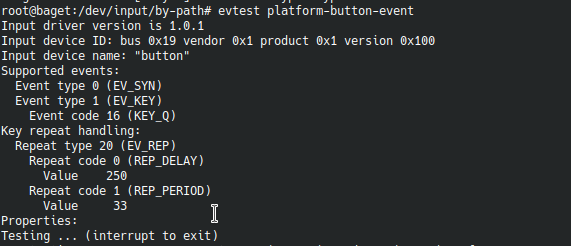
\includegraphics[width=\textwidth]{pic_17}
\end{center}

\subsection{}Нажмите и отпустите кнопку. Вы увидите как в консоли появиться несколько записей. Это информация о событии. 
\begin{center}
	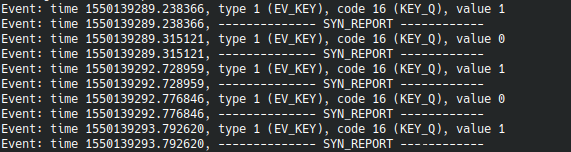
\includegraphics[width=\textwidth]{pic_18}
\end{center}
\textbf{Замечание:} обратите внимание на значение параметра value, оно кодирует состояние кнопки 0 — отпущена, 1 — нажата, 2 — удерживается  

\subsection{}Прервём работу команды, нажав Ctrl+C (рекомендуется её запомнить, при работе с консолью в Linux, эта комбинация используется часто, для прерывания выполнения текущей команды или программы)

\subsection{}Дополнительно посмотрим, что на самом деле считывается из файла при работе с ним, для чего запустим конвейер из двух команд
\begin{lstlisting}[style=bash]
$ cat /dev/input/event0 | hexdump 
\end{lstlisting}
Тут уже при открытии Вы не увидите ничего, однако как только начнёте нажимать и отпускать кнопку, то увидите поток данных. В этом потоке храниться как информация о событии, так и временные метки, что мы видели ранее, инструмент evtest занимается преобразованием (парсингом) этого потока, в человечески воспринимаемый вид. 

\subsection{}Прервём работу нажав Ctrl+C.

\subsection{}Светодиоды управляются через виртуальную файловую систему sysfs. Перейдите в следующий каталог
\begin{lstlisting}[style=bash]
$ cd /sys/class/leds
\end{lstlisting}

\subsection{}Тут располагаются ссылки на все светодиоды доступные в системе. В нашем случае, дожно быть две папки mmc0:: и led1, проверьте выполнив команду  
\begin{lstlisting}[style=bash]
$ ls -l
\end{lstlisting}

\subsection{}Для управления состоянием светодиода отправьте 1 в файл brightness для включения светодиода, и 0 для выключения. При подключении через ШИМ контроллер, этот файл позволяет устанавливать яркость светодиода (например, для управления яркостью подсветки экрана)
\begin{lstlisting}[style=bash]
$ echo 1 > led1/brightness
$ echo 0 > led1/brightness
\end{lstlisting}

\section{Собираем свой драйвер}
Попробуем теперь использовать вывод общего назначения внутри собственного драйвера, что может часто понадобиться, при работе с внешними модулями. К примеру, для управления сигнала сброса, или для переключения между режимами и т. д.

\subsection{}Скопируем код демонстрирующий работу с GPIO в пространстве ядра. Вернитесь в консоль виртуальной машины, и выполните следующую команду, и посмотрим в него 
\begin{lstlisting}[style=bash]
# cp -r $BAGET/support/gpio_driver $BAGET/lab_04/driver
# cd $BAGET/lab_04/driver; code .
\end{lstlisting}
\begin{center}
	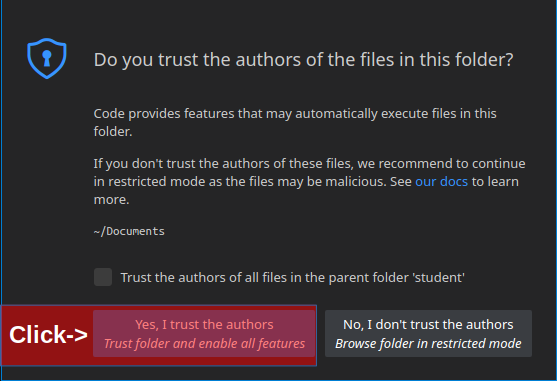
\includegraphics[width=0.5\textwidth]{pic_13}
\end{center}
\textbf{Замечание:} При первом входе, Вас могут спросить, доверяете ли вы автору, нужно нажать на кнопку Yes,  


\subsection{}Добавим путей для разрешения части include директив. Откройте .vscode -> c\_cpp\_properties.json
\begin{center}
	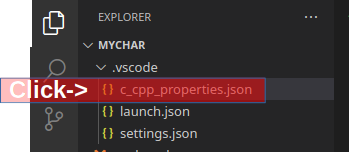
\includegraphics[width=0.5\textwidth]{pic_14}
\end{center}

\subsection{}Допишите в поле includePath следующие строки:\\
\begin{center}
	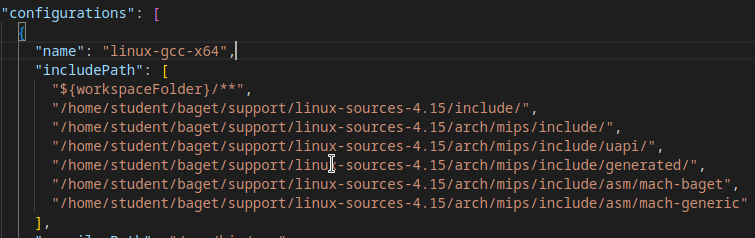
\includegraphics[width=\textwidth]{pic_15}
\end{center}
для удобства, воспользуйтесь файлом vscode\_lines.md в папке support.

Ctrl+S для сохранения.

\subsection{}Допишем compilerArgs, как на картинке ниже, для корректного перехода к реализации функций gpio драйвера ядра.\\
\begin{center}
	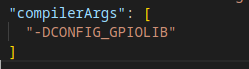
\includegraphics[width=0.5\textwidth]{pic_19}
\end{center}

\subsection{}Посмотрим на содержимое файла gpio\_temp.c. В нём описан процесс подключения драйвера к выводу.

\subsection{}Так же откройте, и посмотрите на Makefile. В нём есть раздел install который поможет Вам скопировать на целевую плату скомпилированный модуль ядра. При этом, перед копированием будет запущена сборка всего проекта. Это полезная практика, так как гарантирует Вам, что при исправлении мелкой опечатки, на плату попадёт код с исправлением, а не его предыдущая версия.

\subsection{}Перейдём в терминал (можно открыть вкладку TERMINAL в vscode, если её не видно, выберите в меню Terminal → New Terminal) и соберём модуль командой:
\begin{lstlisting}[style=bash]
# ARCH=mips CROSS_COMPILE=mips64el-linux-gnuabi64- make 
\end{lstlisting}

\subsection{}Проверьте значение системной переменной BRD\_PASS  
\begin{lstlisting}[style=bash]
# echo $BRD_PASS
\end{lstlisting}
если вывод был пустой, проинициализируйте переменную 
\begin{lstlisting}[style=bash]
# export BRD_PASS="usrnetuser" 
\end{lstlisting}

\subsection{}Скопируйте модуль на плату
\begin{lstlisting}[style=bash]
	# ARCH=mips CROSS_COMPILE=mips64el-linux-gnuabi64- make install
\end{lstlisting}
\textbf{Замечание:} попробуйте сами разобратся, как в Makefile описан процес копирования файла на плату. Это может Вам помочь, при выполнении самостоятельных работ.

\subsection{}Внесите изменения в файл дерева-устройств 
\begin{lstlisting}[style=bash]
# kate $BAGET/lab_04/of_dtb/of_gpio.dts
\end{lstlisting}
удалите ноды led1 и button, и допишите новую ноду:
\begin{lstlisting}[style=stdout]
custom {
	compatible = "gpio,dummy";
	status = "okay";
	yellowled-gpios = <&gpiof 1 0>;
};
\end{lstlisting}
\textbf{Замечание:} обратите внимание на строку, в которой мы указываем информацию о выводе, которым нужно управлять. Первая часть (yellowled…) должна совпадать с той меткой, что указана в исходном коде, на 62 строке!

\subsection{}Сохраните изменения Ctrl+S и закройте редактор Ctrl+Q 

\subsection{}Скомпилируем файл dts, для этого выполним следующую команду
\begin{lstlisting}[style=bash]
# dtc --symbol -O dtb -o $BAGET/lab_04/of_dtb/of_gpio.dtb \
$BAGET/lab_04/of_dtb/of_gpio.dts
\end{lstlisting}

\subsection{}Скопируйте полученный файл на плату
\begin{lstlisting}[style=bash]
# scp $BAGET/lab_04/of_dtb/of_gpio.dtb \
netuser@192.168.100.200:/home/netuser/
\end{lstlisting}

\subsection{}Перейдите в терминал платы, и переместите файл в папку barebox
\begin{lstlisting}[style=bash]
$ mv /home/netuser/*.dtb /barebox/
\end{lstlisting}

\subsection{}Перезагрузите плату командой reboot

\subsection{}После перезагрузки, подгрузите модуль командой
\begin{lstlisting}[style=bash]
$ insmod /home/netuser/gpio_temp.ko
\end{lstlisting}
Если не было допущено ошибок, то в течении 20 секунд плата будет перемигиваться с Вами светодиодами F0 и F1

\subsection{} Выключите плату, для чего в начале введите команду
\begin{lstlisting}[style=bash]
	$ poweroff
\end{lstlisting}
дождитесь, как появиться надпись
\begin{lstlisting}[style=stdout]
	reboot: System halt
\end{lstlisting}
после чего отключите USB кабель от ПК или платы. 

\section{Задание для закрепления}
Измените код таким образом, что бы светодиод начинал мигать, когда кнопка нажата. Для этого воспользуйтесь таймером.

\begin{itemize}
	\item Добавьте функцию инициализирующую кнопку (нужно сделать всё то же, что и при инициализации светодиода, в функции int myled\_init(int gpio\_id), за исключением того, что направления вывода должно быть GPIOD\_INPUT
	
	\item Для считывания состояния кнопки, используйте функцию gpio\_get\_value(<gpio\_id>). Помните, что кнопка на плате имеет инверсную логику, другими словами в отпущенном состоянии вывод прижат к питанию, и возвращает 1.
	
	\item Пример кода по инициализации таймера
	\begin{lstlisting}[style=stdout]
		      #include <linux/module.h> /* Needed by all modules */
		#include <linux/kernel.h> /* Needed for KERN_INFO */
		#include <linux/init.h> /* Needed for the macros */
		#include <linux/timer.h>
		#include <linux/jiffies.h>
		
		int g_time_interval = 250; // miliseconds
		struct timer_list g_timer;
		
		void _TimerHandler(struct timer_list *tm)
		{
			static bool state = true;
			printk("%s: %s", DRIVER_NAME, __func__);
			state = !state;
			mod_timer(tm, jiffies + msecs_to_jiffies(g_time_interval));
		}
		
		static int __init my_init(void)
		{
			printk(KERN_INFO "My module inserted into kernel!!!.\n");
			
			/*Starting the timer.*/
			setup_timer(&g_timer, _TimerHandler, 0);
			mod_timer( &g_timer, jiffies + msecs_to_jiffies(g_time_interval));
			
			return 0;
		}
		
		static void __exit my_exit(void)
		{
			del_timer(&g_timer);
			printk(KERN_INFO "My module exited from kernel!!!\n");
		}
		
		module_init(my_init);
		module_exit(my_exit);
	\end{lstlisting}

	\item не забудьте добавить освобождение ресурсов для кнопки и таймера.
\end{itemize}